\chapter{Grundlagen}
Dieses Kapitel befasst sich mit sowohl den mathematischen als auch den technischen Grundlagen der zu behandelnden Thematik, welche für das weitere Verständnis der Arbeit beitragen. \textit{Auf mobile Anwendungen geht dieses Grundlagenkapitel nicht in besonderer Tiefe ein, da ein allgemeines Verständnis und Vertrautheit mit Konzepten und Technologien mobiler Anwendungen vorausgesetzt wird.}
\section{Mathematische Grundlagen}
\subsection*{Berechnung der Geschwindigkeitsempfehlung}
Präsentiert das System während der Anwendung eine Geschwindigkeitsempfehlung, ist diese abhängig von der Fahrtgeschwindigkeit und vom Abstand zur Ampel. Angenommen die Progressionsgeschwindigkeit $v$ wird zum Zeitpunkt $t_{1}$ ausgesprochen, die \gls {LSA} schaltet zum Zeitpunt $t_{2}$ auf Rot und Abstand zur Ampel beträgt $s$, dann gilt: \\
\[ v = \frac{s}{t_{2} - t_{1}} \] \\
\begin{figure}[H]  
    \centering  
    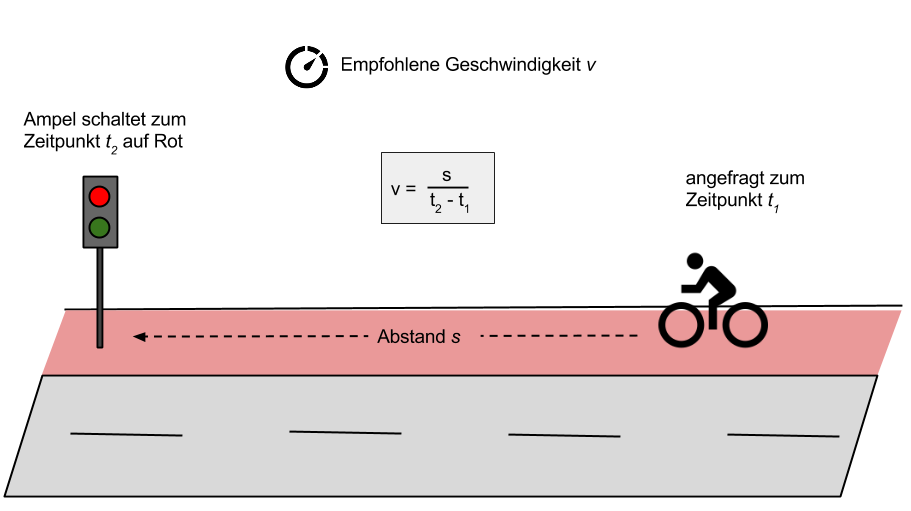
\includegraphics[width=1\textwidth]{vst} 
    \label{fig:szenarien}
    \caption[Berechnung Progressionsgeschwindigkeit]{Berechnung der zu empfehlenden Geschwindigkeit}
\end{figure}
Um die ensprechende \gls{LSA} während der Grünphase zu passieren, muss letztendlich die empfohlene Geschwindigkeit $v$ eingehalten werden. Folgende Fälle werden beachtet:
\begin{figure}[H]  
    \centering  
    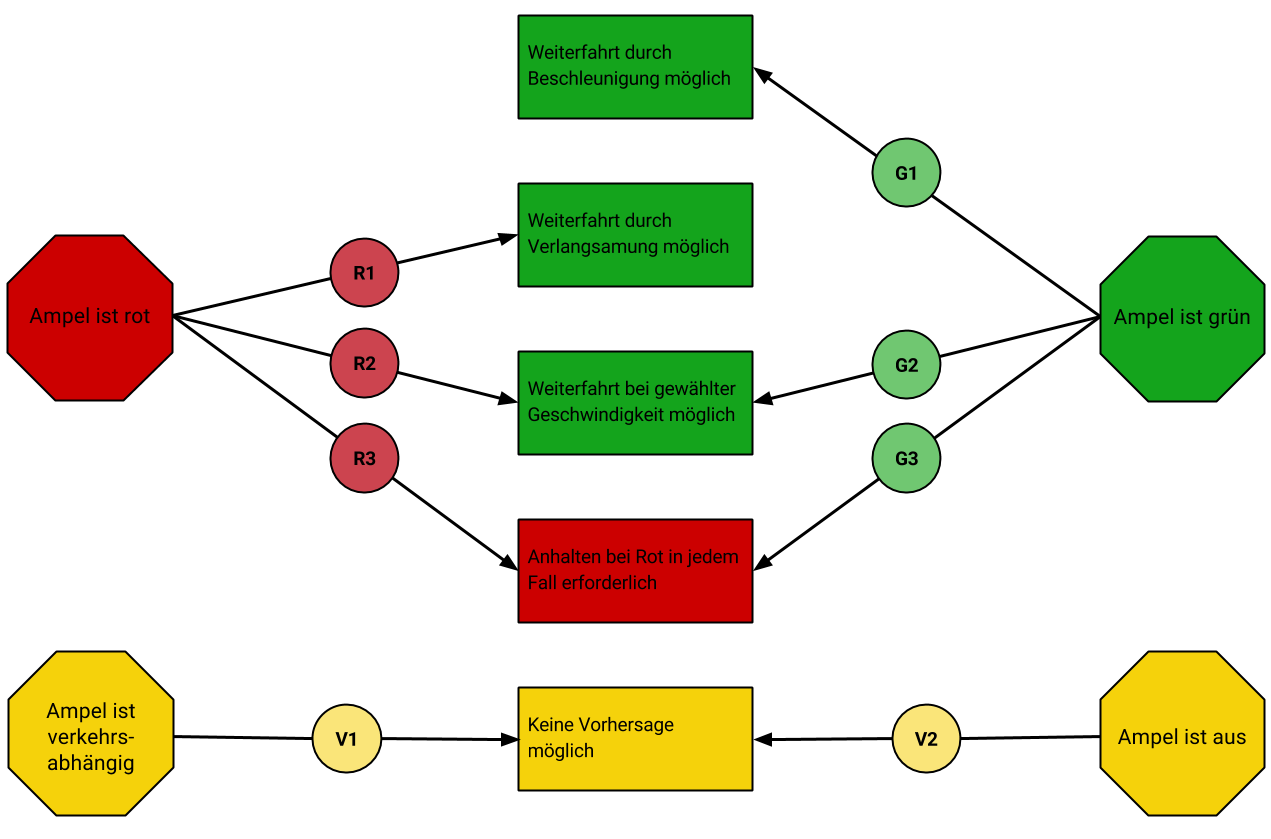
\includegraphics[width=1\textwidth]{Szenarien} 
    \label{fig:szenarien}
    \caption[Szenarien]{Mögliche Szenarien}
\end{figure}
\paragraph{Anhalten ist unvermeidbar:} Die Ampelschaltung erlaubt momentan kein reibungsloses Passieren. 
\textit{Umgesetzte Anzeigevariante: \textbf{rot}}
\paragraph{Konstante Weiterfahrt möglich:} Ist die empfohlene Geschwindigkeit gleich der aktuellen, ist ein reibungsloses Passieren bei beibehaltenem Tempo möglich. Es besteht kein Handlungsbedarf. 
\textit{Umgesetzte Anzeigevariante: \textbf{grün}}
\paragraph{Reibungsloses Passieren durch Beschleunigung möglich:} Zeigt die Ampel im Moment Grün und ist die empfohlene Geschwindigkeit höher als die aktuelle, ist ein reibungsloses Passieren durch Beschleunigung zu erreichen. Bei der Anzeige der Progressionsgeschwindigkeit ist selbstverständlich die geltende Höchstgeschwindigkeitsbegrenzung zu beachten. 
\textit{Umgesetzte Anzeigevariante: \textbf{grün}}
\paragraph{Reibungsloses Passieren duch Verlangsamen möglich:} Zeigt die Ampel im Moment Rot und ist die empfohlene Geschwindigkeit niedriger als die aktuelle, ist ein reibungsloses Passieren durch Verlangsamung zu erreichen.
\textit{Umgesetzte Anzeigevariante: \textbf{grün}}
%\subsection{Berechnung der Restrotanzeige}
% ist aber trivial
% -------------------------------------------------
% TECHNISCHE GRUNDLAGEN
% -------------------------------------------------
\section{Technische Grundlagen}
Im folgenden Abschnitt werden Funktionsweise und Besonderheiten der verwendeten Technologien beschrieben.
% ANDROID
\subsection{Android}
\subsubsection{Mobile Sensing}
\subsection{SQLite}
